\chapter{Undecidability}

\section{The Diagonalization Method}

Cantor (\~1890s) had the following idea:
\begin{definition}[Same size of sets]
    Say that set \(A\) and \(B\) \underline{have the same size} if there is a one-to-one("injective") and \textbf{onto}("surjective") function: \(f: A \rightarrow B\).   
\end{definition}

\begin{example}[Countable Sets]
    Let \(N = \{ 1, 2, 3, \cdots \} \)  and let \(Z = \{ \cdots, -2, -1, 0, 1, 2, \cdots \} \). Show \(N\) and \(Z\) have the same size.  
\end{example}

\begin{example}[Countable Sets]
    Let \(Q^+ = \{ m/n  | m, n \in N\} \), show \(N\)  and \(Q^+\) has the same size.  
\end{example}

\begin{definition}[Countable]
    A set \(A\) is countable if either it is finite or it has the same size as \(\mathbb{N} \). 
\end{definition}

\begin{theorem}[\(\mathbb{R}\)  is Uncountable]
    Let \(\mathbb{R}\) = all real numbers 
\end{theorem}
\begin{proof}
   Proof by contradiction via diagonalization: Assume R is countable. 

   So there is a 1-1 correspondence \(f: N \rightarrow R\) 

   Demonstrate a number \(x \in R\) that is missing from the list. It has i-th digit different from the i-th number in the list. 

   \begin{figure}[H]
   \centering
   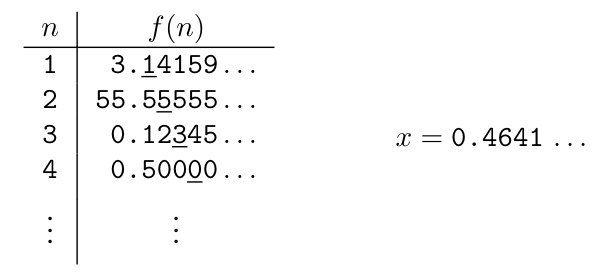
\includegraphics[width=0.8\textwidth]{l8.1.jpg}
   \caption{Diagonalization}
   \end{figure}
\end{proof}


Let L = all languages, we have some corollaries:
\begin{corollary}
    L is uncountable.
\end{corollary}
\begin{proof}
    There's a 1-1 correspondence form L to R so they are the same size.

    \begin{remark}[Observation]
        \(\Sigma^* = \{ \epsilon, 0, 1, 00, 01, 10, 11, 000, \cdots \} \) is countable. 

        For each length, there are only finite numbers of strings.
    \end{remark}
    \begin{remark}[Observation]
        The set of all Turing machines is countable because each Turing machine M has an encoding into a string \(\langle M \rangle\). 

        \textbf{Why each M can encode?}: Because TM is a finite object with a well-defined structure. \begin{quote}
            A Turing machine M can be described as a 7-tuple \(Q, F, q_0, \Sigma, \Gamma, \delta, blank \). 
            This means that if someone gives you this 7-tuple, then the TM is well-defined, and you can precisely define how it behaves, etc.
            (\href{https://cs.stackexchange.com/a/49616/177809}{CSStackExchange})
        \end{quote}
        
        \textbf{Why this mean M is countable?}: This is my thought, because each TM can be encoded into a string. And because the encoding alphabet of the string is limited, for the same reason why \(\Sigma^*\) is countable, this is also countable. 
    \end{remark}

    \begin{theorem}
        The set of all infinite binary sequences is uncountable.
    \end{theorem}
    \begin{proof}
        This is easy to be proved by using diagonalization.
    \end{proof}

    Let \(\mathcal{B}\) be the set of all infinite binary sequences. 
    We can show that the set of all languages \(\mathcal{L}\) has the same size of \(\mathcal{B}\):

    \begin{figure}[H]
    \centering
    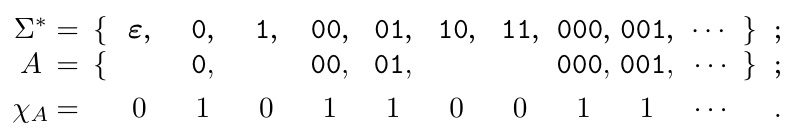
\includegraphics[width=0.8\textwidth]{l8.2.jpg}
    \end{figure}

    For each kind of language \(A\), according to whether a string exists in it, we can generate a bitmap \(\mathcal{X}_A\) according to that.  
\end{proof}

\begin{corollary}
    Some language is not decidable 
\end{corollary}
\begin{proof}
    There are more languages than Turing Machine! 
\end{proof}

\begin{remark}
    Consider Hilbert's 1st question.
\end{remark}

\section{Undecidable Language}
\begin{theorem}\label{theorem: undecidable language}
    \(A_{TM}\) = \{ \(\langle M, w \rangle\) | \(M\) is a TM and \(M\) accepts \(w\)  \} 

    \(A_{TM}\) is not decidable. 
\end{theorem}
\begin{proof}
    Assume some TM \(H\) decides \(A_{TM}\).  

    So \(H\) on \(\langle M, w \rangle = \) \begin{align*}
        & Accept \; if \; M \;accepts \;w\\
        & Reject \; if \; not
    \end{align*} 

    Use \(H\) to construct TM \(D\)  

    D = "On input \(\langle M \rangle \)
        \begin{enumerate}
            \item Simulate \(H\) on input \(\langle M \langle M \rangle \rangle \)
            \item \(Accept\) if H rejects, \(Reject\) if H accepts."    
        \end{enumerate} 

    \(D\) accepts \(\langle M \rangle \) iff \(M\) doesn't accept \(\langle M \rangle\).    

    \(D\) accepts \(\langle D \rangle \) iff \(D\) doesn't accept \(\langle D \rangle\).    

    Contradiction.
    \hfill\break

    \textbf{Where is the diagonalization?}
    \begin{figure}[H]
    \centering
    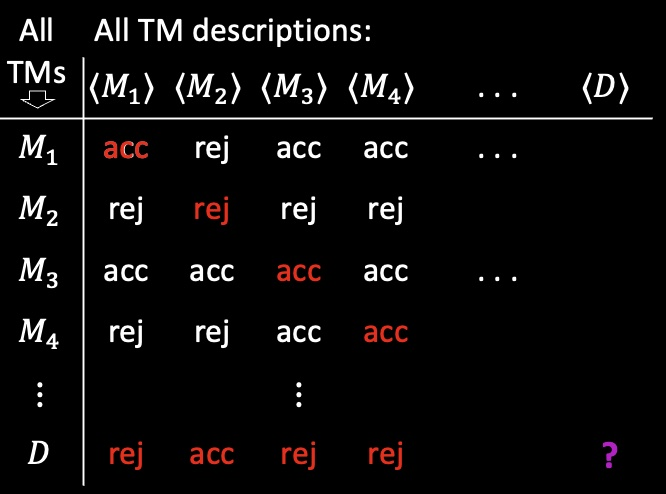
\includegraphics[width=0.6\textwidth]{l8.3.jpg}
    \caption{}
    \end{figure}
\end{proof}

This implies that there is no TM that can always decide whether an arbitrary TM M  will accept an input w. 

\begin{theorem}
    If \(A\)  and \(\overline{A}\) are T-recognizable then \(A\) is decidable. 
\end{theorem}

This theorem connects decidability and recognizability.

\begin{proof}
    Let TM \(M_1\) and \(M_2\) recognize \(A\) and \(\overline{A}\).     

    Construct TM \(T\) deciding A. 

    \(T = \) "On input \(w\)
    \begin{enumerate}
        \item Run \(M_1\) and \(M_2\) on \(w\) in parallel until one accepts.
        \item If \(M_1\) accepts then \(accept\), if \(M_2\) accepts then reject. "
    \end{enumerate}  
\end{proof}

\begin{corollary}
    \(\overline{A_{TM}}\) is T-unrecognizable. 
\end{corollary}
\begin{proof}
    \(A_{TM}\) is T-recognizable but also undecidable (as we have proved \hyperref[theorem: undecidable language]{here}). 
    If \(\overline{A_{TM}}\) is also recognizable, then \(A_{TM}\) should be decidable.  
\end{proof}

Here is the relationship:
    \begin{figure}[H]
    \centering
    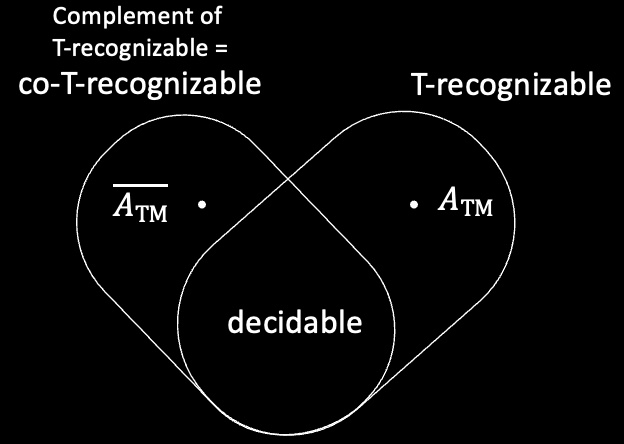
\includegraphics[width=0.8\textwidth]{l8.4.jpg}
    \caption{}
    \end{figure}

\section{The Reducibility Method}

Use our knowledge that \(A_{TM}\) is undecidable to show other problems are undecidable. 

\begin{definition}
    \(HALT_{TM}\) = \{ \( \langle M, w \rangle\) | \(M\) halts on input \(w\) \}  
\end{definition}

\begin{theorem}
    \(HALT_{TM}\) is undecidable. 
\end{theorem}
\begin{proof}
    Assume that \(HALT_{TM}\) is decidable and show that \(A_{TM}\) is decidable (false!)  

    \(A_{TM} \) is undecidable has been proved in \hyperref[theorem: undecidable language]{here}.

    Let TM \(R\) decide \(HALT_{TM}\).
    
    Construct TM \(S\) deciding \(A_{TM}\).  

    \(S = \) "On input \(\langle M, w \rangle\) 
        \begin{enumerate}
            \item Use R to test if M on w halts, if not, reject.
            \item Simulate M on w until it halts (as guaranteed by R)
            \item If M has accepted then \(accept\), if M has rejected then \(reject\)."
        \end{enumerate} 

    TM \(S\) decides \(A_{TM}\), a contradiction. Therefore \(HALT_{TM}\) is undecidable.   
\end{proof}


